


\subsection{Reformulation of the flux, Interphase terms and fluid mediated interactions.} 


\subsubsection{The flux reformulation}

One of the problem encountered in the classic two fluid formulation of the momentum equation is that the averaged pressure terms $\phi_1 p_1$  appear under the gradient operator. 
Under this form this terms leads to physical behavior \citet{jackson2000}.
Consequently, we reformulate the flux and exchange terms of \ref{eq:dt_avg_rho} and \ref{eq:dt_avg_rhoE_k} following these relations, 
\begin{align*}
    \avg{\delta_I \bm{\sigma}_1^0  \cdot \textbf{n}_2} + \grad (p_1 \phi_1)
    &\approx 
    + \phi_1 \grad p_1
    + \avg{\delta_I \bm{\sigma}_1'\cdot \textbf{n}_2}
    \\
    \avg{\delta_I  \textbf{q}_2 \cdot \textbf{n}_2} - \div (\textbf{q}_1\phi_1)
    &\approx 
    \phi_1 \grad(\textbf{q}_1)
    + \avg{\delta_I \textbf{q}_1' \cdot \textbf{n}_2}\\
    \avg{\delta_I (\textbf{u}_1^0 \cdot\bm{\sigma}_1^0 )\cdot \textbf{n}_2} - \div (\textbf{u}_1p_1\phi_1)
    % = \avg{\delta_I (\textbf{u}_1 \cdot \bm{\sigma}_1' + \textbf{u}_1' \cdot \bm{\sigma}_1^0 )\cdot \textbf{n}_2}
    &\approx 
    \phi_1 \grad(\textbf{u}_1 p_1)
    + \textbf{u}_1 \cdot \avg{\delta_I \bm{\sigma}_1'\cdot \textbf{n}_2}
    + \avg{\delta_I (\textbf{u}_1' \cdot \bm{\sigma}_1^0 )\cdot \textbf{n}_2}
\end{align*}
where $\bm{\sigma}_1' = \bm{\sigma}_1^0 + p_1 \textbf{I}$ is the stress over the surface of the particle, minus the contribution from the mean pressure gradient which is accounted by the term, $\phi_1\grad p_1$. 




% On the fluid side equations (\ref{eq:dt_avg_rho}, \ref{eq:eq:dt_avg_rho_ku})
% Before exposing the complete system for dispersed two-phase flow equations we make a brief points on the exchanges terms reformulation. 
\subsubsection{Particle and continuous inter phase phase exchange terms}

Now that we retrieve the mean flux to the different exchanges terms we must expand them as particle terms to be consistent with the particle phase equations. 
Indeed, to reach conciseness, the exchange terms on the continuous phase conservation equation of the form of : (\ref{eq:avg_dt_chi_f}), must be the same as for the particle phase equations (\ref{eq:avg_dt_dq_alpha_tot} and \ref{eq:avg_dt_dq_alpha_tot}). 
However, in the latter we find interfacial averaged term in the form of $\avg{\delta_I \ldots}$ and on the other we find particle averaged term such that $\pnnavg{\intS{\ldots}}$. 
Therefore, on the fluid side equations we must expand the terms in a series following \ref{eq:f_exp} to be well consistent.
For the momentum and energy equations it reads, 
\begin{align*}
    \avg{\delta_I \bm{\sigma}_1'\cdot \textbf{n}_2}
    &=
    \pavg{\intO{\bm{\sigma}_1'\cdot \textbf{n}_2}}
    - \div 
    = \pavg{\intO{\textbf{r}\bm{\sigma}_1'\cdot \textbf{n}_2}}
    = 
    n_p \textbf{f}_p
    -\div (n_p \textbf{F}_p)\\
    \avg{\delta_I (\textbf{u}_1' \cdot \bm{\sigma}_1^0 )\cdot \textbf{n}_2}
    &=
    \pavg{\intS{\textbf{u}_1' \cdot \bm{\sigma}_1^0 \cdot \textbf{n}_2}}
    -\div \pavg{\intS{\textbf{r}\textbf{u}_1' \cdot \bm{\sigma}_1^0 \cdot \textbf{n}_2}}
    = 
    n_p \textbf{c}_p
    -\div (n_p \textbf{C}_p)\\
    \avg{\delta_I \textbf{q}_1' \cdot \textbf{n}_2}
    &=
    \pavg{\intS{\textbf{q}_1' \cdot \textbf{n}_2}}
    - \div \pavg{\intS{\textbf{r}\textbf{q}_1' \cdot \textbf{n}_2}}
    =
    n_p \textbf{q}_p
    -\div (n_p \textbf{Q}_p)
\end{align*}
where we introduce $\textbf{f}_p$, $\textbf{c}_p$ and $\textbf{q}_p$ as the particle averaged drag force, work due to local forces over the surface of the particle and heat flux, respectively. 
Additionally, under the divergence sign we observe the terms $\textbf{F}_p$, $\textbf{C}_p$ and $\textbf{Q}_p$ which are the first moment of the hydrodynamic force, work of the surface force and heat flux. 

On the particles phase equations it can be demonstrated that similar relations holds to retrieve the mean flux contribution to the exchange terms.
For the drag force and first moment of the drag force we have the following relations :
\begin{align*}
    \pavg{\intS{\bm{\sigma}^0_1 \cdot \textbf{n}_2}}
    \approx
    n_p \textbf{f}_p
    - n_p v_p \grad p_1,\\
    \pavg{\intS{\textbf{r}\bm{\sigma}^0_1 \cdot \textbf{n}_2}}
    \approx
    n_p \textbf{F}_p
    - n_p v_p p_1 \textbf{I}.
\end{align*}
Similar relations can be found to recover the others terms appearing in the fluid phase equations. 
Unlike the previous equations, these relations are not exact to $\mathcal{O}(a/L)$. 

\subsubsection{Fluid mediated interactions and nearest-neighbors statistics}

In this section we would like to separate fluid mediated interaction such as lubrication forces or in the case of droplets surface tension forces from the drag force term $\textbf{f}_p$.  

From \citet{nott2011suspension} and more recently \citet{zhang2021ensemble} it has been demonstrated that it is possible to separate the mean drag force term $\textbf{f}_p$ into a binary or pure drag force term : $\textbf{f}_\text{pm}$, and the divergence of a second order tensor called the particle-fluid-particle stress : $\textbf{F}_\text{pfp}$. 
To be more specific $\textbf{f}_p n_p  = n_p \textbf{f}_\text{pm} + \div (n_p \textbf{F}_\text{pfp})$. 
This tensor account for long and short range interaction between particles through the ambient phase. 
It can be through as the correlation between the force experienced by the particles and the position of its nearest neighbor. 
It describes the particle phase pressure. 
This terms must be accounted in our model since it has been shown to be circuital to obtain a hyperbolic equation of momentum \citep{fox2020hyperbolic}. 

Note that following the methodology of \citet{zhang2021ensemble} any particle averaged terms could be expanded following the decomposition of the drag force term. 
However, the first order terms are relevant only if the particle quantity is correlated with the position of its neighboring particles.  
For the heat flux it would imply that a particle would receive more heat due to the close presence of another particles. 
For simplicity, we will consider that it is only the case for the drag force term. 
\tb{maybe look at pathz to expose like him}

\subsection{Continuous phase equations}


\subsubsection{Primary equations}

We start by exposing the continuous phase primary equation. 
They are simply derived using the general formulation \ref{eq:avg_dt_chi_f} and using the preceding remarks. 
Applying the above methodology, we express the mass, momentum and total energy of the continuous phase yielding, 
\begin{align}
    \label{eq:dt_hybrid_rho_1}
    \pddt (\phi_1 \rho_1)  
    + \div (
        \phi_1 \rho_1\textbf{u}_1
    )
    &= 
    0\\
    \label{eq:dt_hybrid_rho_1u_1}
    \pddt (\phi_1 \rho_1\textbf{u}_1)  
    + \div (
        \phi_1 \rho_1\textbf{u}_1\textbf{u}_1
        + \bm{\sigma}_1^\text{eq}
    )
    &= 
    \phi_1 (\rho_1 \textbf{g} 
    - \grad p_1 ) 
    -  n_p \textbf{f}_\text{pm}\\
    \label{eq:dt_hybrid_rho_1E_1}
    \pddt (\phi_1\rho_1E_1)  
    + \div (
        \phi_1\rho_1E_1\textbf{u}_1
        + \bm{q}_1^\text{eq}
        + \textbf{u}_1 \cdot \bm{\sigma}_1^\text{eq}
        )
    &= 
    n_p (\textbf{F}_\text{pfp}- \textbf{F}_p) :\grad \textbf{u}_1
    +\phi_1 [\rho_1\textbf{u}_1 \cdot \textbf{g} 
    - \div(\textbf{u}_1p_1 + \textbf{q}_1)]\nonumber\\
    &- n_p \textbf{u}_1 \cdot \textbf{f}_\text{pm}
    - n_p \textbf{c}_p
    + n_p \textbf{q}_p
\end{align} 
where we defined the equivalent stress tensor $\bm{\sigma}_1^\text{eq}$ and energy flux $\textbf{q}^\text{eq}_1$ as,
\begin{align*}
    &\bm{\sigma}_1^\text{eq}
    = \phi_1\rho_1\oneavg{\textbf{u}_1'\textbf{u}_1'}
    - \bm{\tau}_1 \phi_1
    + n_p (\textbf{F}_\text{pfp} - \textbf{F}_\text{p})
    &\textbf{q}_1^\text{eq}
    =\textbf{q}_1^\text{e} +\textbf{q}_1^\text{k} \\
    &\textbf{q}_1^\text{e}
    = \phi_1\rho_1 \oneavg{\textbf{u}_1' e_1'} + n_p \mathbf{Q}_p
    &\textbf{q}_1^\text{k}
    = \phi_1\rho_1 \oneavg{\textbf{u}_1' k_1} 
    - \phi_1\oneavg{\textbf{u}_1' \cdot \bm{\sigma}_1^0}
    - n_p \textbf{C}_p 
\end{align*}
\tb{Thinck about the exchange terms $\textbf{c}_p$ in faxen form }
It is clear that those equations yield essentially the same as the previous set of equations except for the exchanges terms modifications.
It is interesting to notice the appearing of $\textbf{F}_\text{pfp}$ and $\textbf{F}_p$ as a diffusive term in  \ref{eq:dt_hybrid_rho_1E_1}.
\todo[inline]{make bibliography and comparaison} 

\subsubsection{Secondary equations}

In light of \ref{eq:E_def} the total energy equation must be completed by using eigher one of the following sub equations, 
\begin{align}
    \pddt (\phi_1 \rho_1u_1^2/2)  
    + \div (
        \phi_1 \rho_1\textbf{u}_1u_1^2/2
        + \textbf{u}_1 \cdot \bm{\sigma}_1^\text{eq}
    )
    &= 
    + \bm{\sigma}_1^\text{eq} : \grad \textbf{u}_1
    + \phi_1  \textbf{u}_1\cdot(\rho_1 \textbf{g} - \grad p_1) 
    - n_p \textbf{u}_1\cdot \textbf{f}_\text{p}\\
    \label{eq:dt_hybrid_k1}
    \pddt (\phi_1\rho_1k_1)  
    + \div (
        \phi_1\rho_1k_1\textbf{u}_1
        + \textbf{q}_1^\text{k} 
        )
    &= 
    - \phi_1\textbf{d}_1
    + \phi_1(\bm{\sigma}_1 - \rho_1 \oneavg{\textbf{u}_1'\textbf{u}_1'} ): \grad \textbf{u}_1
    - n_p \textbf{c}_p\\
    \pddt (\phi_1\rho_1e_1)  
    + \div (
        \phi_1 \rho_1e_1\textbf{u}_1
        +
        \textbf{q}_1^\text{e} 
        )
    &= 
    \phi_1\textbf{d}_1
    - \phi_1 \div \textbf{q}_1
    + n_p \textbf{q}_p
\end{align}
where we introduced the averaged local dissipation tensor $\textbf{d}_1 = \oneavg{\bm{\sigma}_1^0 : \grad \textbf{u}_1^0}$. 
It is interesting to notice that in \ref{eq:dt_hybrid_k1} nor the first moment of hydrodynamic forces $\textbf{F}_p$ nor the particle-fluid-particle stress $\textbf{F}_\text{pfp}$ appear under the macroscopic sink term. 
The only additional flux is $n_p \textbf{C}_p$, which is the first moment of the surface correlation of the work of the local forces. 
Similar comments hold for the  internal energy. 

Usually one would need only two of the energy equations, usually the equation of $k_1$ and $e_1$.
Therefore, closure must be provided for both equations. 


\subsection{Dispersed phase equations}

\subsubsection{Primary equations}

Regarding the dispersed phase we have :
\begin{align}
    \label{eq:dt_hybrid_mp}
    \pddt \left(n_p m_p\right)
    + \div \left(n_pm_p\textbf{u}_p
    \right)
    &= 
    0\\
    \label{eq:dt_hybrid_up}
    \pddt \left(n_p m_p \textbf{u}_p\right)
    + \div \left(n_p
    m_p \textbf{u}_p \textbf{u}_p 
    + \bm{\sigma}_p^\text{eq}
    \right)
    &= 
    n_p v_p (\rho_2 \textbf{g}
    - \grad p_1)
    + n_p \textbf{f}_{pm},\\
    \label{eq:dt_hybrid_Ep}
    \pddt(m_p n_pE_p^\text{tot})
    + \div(m_pn_p E_p^\text{tot} \textbf{u}_p 
    + \textbf{q}_p^\text{eq} 
    + \textbf{u}_p \cdot \bm{\sigma}_p^\text{eq})
    &= n_p (\textbf{F}_p -\textbf{F}_\text{pfp}): \grad \textbf{u}_1 \\
    + n_p v_p [\rho_2 \textbf{u}_p\cdot  \textbf{g}
    - \div (\textbf{u}_1 p_1 + \textbf{q}_1)]
    % +  n_p ( \textbf{u}'_1 \cdot \bm{\sigma}_1^0 \cdot \textbf{n}_2)_p^\Sigma
    &-  n_p \textbf{q}_p
    +  n_p \textbf{u}_1 \cdot \textbf{f}_{pm}
    +  n_p \textbf{c}_p
\end{align}
\begin{align*}
    &\bm{\sigma}_p^\text{eq}
    = m_p\pnavg{\textbf{u}_\alpha'\textbf{u}_\alpha'} 
    - n_p \textbf{F}_\text{pfp} 
    &\textbf{q}_p^\text{eq}
    =\textbf{q}_p^\text{e} 
    +\textbf{q}_p^\text{k}  
    +\textbf{q}_p^\text{w}  
    \\
    &\textbf{q}_1^\text{e}
    = m_p \pnavg{\textbf{u}_\alpha' e_\alpha'} 
    &\textbf{q}_p^\text{k}
    = m_p \pnavg{\textbf{u}_\alpha' k_\alpha} 
    \\
    &\textbf{q}_p^\text{w}
    = 
    + \pnavg{\textbf{u}_\alpha'(\rho_2 (w^0_2)^2/2 )'_\Omega}
    + \gamma \pnavg{\textbf{u}_\alpha' s_\alpha'}
    - n_p (\textbf{u}_1 - \textbf{u}_p)\cdot \textbf{F}_\text{pfp}
\end{align*}
Here too we observe the first moment and fluid particle stress appearing. 
It is exchange terms appear due to the manipulation of the exchange term. 

\subsubsection{Secondary equations}

For the particle phase the energy decomposition is somewhat more involving. 
It reads, 
\begin{equation*}
    n_p m_p E_p(t) 
    = m_p n_p e_p 
    + n_p W_p
    + m_p n_p k_p
    + m_p n_p (u_p)^2/2
\end{equation*}
where we have introduced the internal kinetic energy with $n_pW_p = \pnavg{\intO{\rho_2  (w_2^0)^2/2}}
+ n_p s_p \gamma$
Each of these terms have a clear meaning. 
Form left to right we find : The internal energy, the internal kinetic energy, the surface energy, the granular temperature and the mean kinetic energy. 

Applying the average procedure on \ref{eq:dt_e_alpha}, \ref{eq:dt_w2_alpha} and \ref{eq:dt_u2_alpha} one can derive an equation for the particle averaged internal energy, internal kinetic energy and mean kinetic energy, it yields, 
\begin{align}
    \label{eq:dt_hybrid_u2p}
    &\pddt \left(n_p m_p (u_\alpha^2)_p/ 2\right)
    + \div \left(n_p
    m_p (u_\alpha^2)_p/ 2 \textbf{u}_p 
    + \textbf{q}^k_p
    + \textbf{u}_p \cdot \bm{\sigma}_p^\text{eq}
    \right)
    = 
    - \textbf{F}_\text{pfp} : \nabla \textbf{u}_p
    + n_p v_p \textbf{u}_p \cdot
    (\rho_2 \textbf{g} - \grad p_1)  \nonumber\\
    &+ n_p\textbf{u}_p \cdot \textbf{f}_\text{pm}
    +n_p(\textbf{u}_\alpha'\cdot(\bm{\sigma}_1^0 \cdot \textbf{n}_2)^\Sigma)_p
    \\
    \label{eq:dt_hybrid_w2p}
    &\pddt \left(n_p W_p\right)
    + \div 
    (n_p W_p
    \textbf{u}_p 
    +  \textbf{q}_p^\text{w}
    )
    = 
    - n_p \textbf{d}_p
    +n_p (\textbf{u}_1 - \textbf{u}_p)  \cdot \textbf{f}_\text{pm}
    - n_p \textbf{F}_\text{pfp} : \grad \textbf{u}_p\nonumber
    + n_p (\textbf{F}_p-\textbf{F}_\text{pfp}) : \grad \textbf{u}_1\\
    &+ n_p \textbf{u}_p \cdot  v_p\grad p_1
    - n_pv_p \div (p_1 \textbf{u}_1)
    + \textbf{c}_p
    - n_p(\textbf{u}_\alpha'\cdot(\bm{\sigma}_1^0 \cdot \textbf{n}_2)^\Sigma)_p\\
    \label{eq:dt_hybrid_ep}
    &\pddt \left(n_p m_p e_p\right)
    + \div \left(n_p
    m_p e_p \textbf{u}_p 
    +  \textbf{q}_p^\text{e}
    \right)
    = 
    + n_p \textbf{d}_p
    - n_p v_p \div \textbf{q}_1
    - n_p \textbf{q}_p
\end{align}


Additionally, taking the dot product of \ref{eq:dt_hybrid_up} with $\textbf{u}_p$ one obtain, 
\begin{equation}
    \label{eq:dt_hybrid_up2}
    \pddt \left(n_p m_p u_p^2/ 2\right)
    + \div \left(n_p
    m_p u_p^2/ 2 \textbf{u}_p 
    + \textbf{u}_p \cdot \bm{\sigma}_p^\text{eq}
    \right)
    = 
     \bm{\sigma}_p^\text{eq}  :\grad \textbf{u}_p
    +  n_p v_p \textbf{u}_p \cdot 
    (\rho_2 \textbf{g} - \grad p_1)
    + n_p \textbf{u}_p \cdot \textbf{f}_{pm},\\
\end{equation}
which is the mean kinetic energy equations. 
Finally by substracting \ref{eq:dt_hybrid_up2} to \ref{eq:dt_hybrid_u2p} we obtain the granular temperature equation :
\begin{multline}
    \label{eq:dt_hybrid_kp}
    \pddt(m_p n_pk_p)
    + \div(m_pn_p k_p \textbf{u}_p 
    + \textbf{q}_p^\text{k})
    = 
     - \bm{\sigma}_p^\text{Re} :\grad \textbf{u}_p
     + n_p (\textbf{u}_\alpha' \cdot (\bm{\sigma}_1^0 \cdot  \textbf{n}_2)^\Sigma)_p
    \\
\end{multline}
remark that this equation is consistent with the usual granular temperature equations derived using kinetic theory. 
One can verify that summing \ref{eq:dt_hybrid_ep}, \ref{eq:dt_hybrid_w2p} and \ref{eq:dt_hybrid_kp} and \ref{eq:dt_hybrid_up2} makes \ref{eq:dt_hybrid_Ep}.  

Under this form we clearly see the fomr of the terms which are in the energy cascade. 
Indeed, the source term $\bm{\sigma}_p^\text{Re} :\grad \textbf{u}_p$ appear in \ref{eq:dt_hybrid_up2} and \ref{eq:dt_hybrid_k1} with opposite sign. 
Consequently, macroscopic kinetic energy is transmitted to granular agitation through the macroscopic diffusion scalar : $\bm{\sigma}_p^\text{Re} :\grad \textbf{u}_p$. 
Then from \ref{eq:dt_hybrid_kp} to \ref{eq:dt_hybrid_w2p} the common term is 
$(\textbf{u}_\alpha' \cdot (\bm{\sigma}_1^0 \cdot  \textbf{n}_2)^\Sigma)_p$. 
Meaning that granular agitation is converted to internal agitation energy through the velocity for covariance term. 
Then among the term appearing in \ref{eq:dt_hybrid_w2p} only the diffusion term $\textbf{d}_1$ is common with  the internal energy equation. 

The remaining terms are the exchange term with the continuous phase. 
To summarize this quite complicated energy cascade we propose this scheme :
\begin{center}
    \tikzstyle{quadri}=[rectangle,draw]
    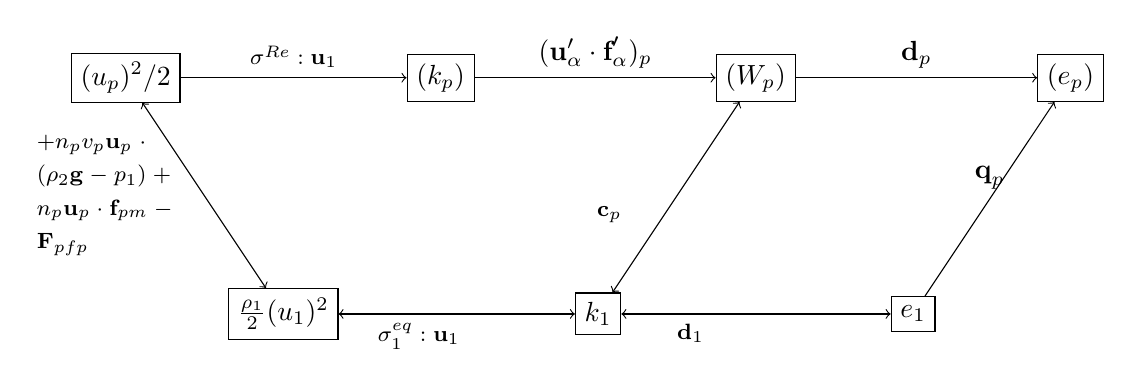
\begin{tikzpicture}
        \node[quadri] (u2) at (0,0){$(u_p)^2 / 2$};
        \node[quadri] (kp) at (4,0){$(k_p)$};
        \node[quadri] (Wp) at (8,0){$(W_p)$};
        \node[quadri] (ep) at (12,0){$(e_p)$};
        \node[quadri] (u12) at (2,-3){$\frac{\rho_1}{2}(u_1)^2$};
        \node[quadri] (k1) at (6,-3){$k_1$};
        \node[quadri] (e1) at (10,-3){$e_1$};
        \draw[->] (u2)--(kp)node[midway,above]{\footnotesize $\bm{\sigma}^\text{Re}:\grad \textbf{u}_1$};
        \draw[<->,text width=2cm] (u2)--(u12) node[midway,left]{\footnotesize $+  n_p v_p \textbf{u}_p \cdot 
        (\rho_2 \textbf{g} - \grad p_1)
        + n_p \textbf{u}_p \cdot \textbf{f}_{pm} - \textbf{F}_\text{pfp}$};
        % \draw[<->,text width=2cm] (kp)--(u12) node[midway,left]{\footnotesize $+  n_p v_p \textbf{u}_p \cdot 
        % (\rho_2 \textbf{g} - \grad p_1)
        % + n_p \textbf{u}_p \cdot \textbf{f}_{pm} - \textbf{F}_\text{pfp}$};
        \draw[<->,text width=2cm] (k1)--(u12) node[midway,below]{\footnotesize $\bm{\sigma}^\text{eq}_1:\grad \textbf{u}_1$};
        \draw[<->,text width=2cm] (k1)--(e1) node[midway,below]{\footnotesize $\textbf{d}_1$};
        \draw[<->,text width=2cm] (k1)--(Wp) node[midway,below]{\footnotesize $\textbf{c}_p$};
        \draw[->] (kp)--(Wp)node[midway,above]{$(\textbf{u}_\alpha' \cdot \textbf{f}_\alpha')_p$};
        \draw[->] (Wp)--(ep)node[midway,above]{$\textbf{d}_p$};
        \draw[->] (e1)--(ep)node[midway,above]{$\textbf{q}_p$};
    \end{tikzpicture}
\end{center}
Nevertheless, under this form the equation lose its meaning. 


\subsection{The first order momentum equations}

Finnaly, if additional information are needed, regarding the internal aspect of the particle. 
As it is suggested by the above equations of energy one can derive the higher moment equations of mass and velocity. 
If one need to solve for additional degree of freedom of the particle one can use the first order moment of momentum and first order moment of mass averaged equaiton which yields, 
\begin{align}
    \pddt \left(n_p \mathcal{M}_p\right)
    + \div \left(
        n_p \textbf{u}_p \mathcal{M}_p
    + \mathcal{M}_p^\text{eq}
    \right)
    &=
    n_p \mathcal{S}_p\\
    \label{eq:dt_hybrid_Pp}
    \pddt \left(n_p \mathcal{P}_p\right)
    + \div \left(
        n_p \textbf{u}_p \mathcal{P}_p
    + \mathcal{P}_p^\text{eq}
    \right)
    &=
    -n_p v_p p_1 \textbf{I}
    + n_p \mathcal{F}_p
    + \left(
        \rho_2 \textbf{w}_2^0  \textbf{w}_2^0 
        - \bm{\sigma}_2'
    \right)^\Omega_p
    - n_p (\gamma \textbf{I}_{||})^\Sigma_p,
\end{align}
This set of equation is complicated. 
We now have a complete set of equation describing the internal kinetic of the particle. 



As remarked by \citet{jackson1997locally} for the angular momentum equations of solid spherical particles, and here in a more general case :\ref{eq:dt_hybrid_rho_1u_1} and \ref{eq:dt_hybrid_up} may seem to be not coupled with the higher order moments equations, i.e. \ref{eq:dt_hybrid_Pp}. 
Indeed, the first order moment $\mathcal{Q}_\alpha$ do not appear explicitly in either \ref{eq:hybrid_avg_dt_chif} or \ref{eq:avg_dt_dq_alpha_tot}.
However, the exchange terms 
$\textbf{f}_p$ 
and 
$\textbf{F}_p$ 
appearing in both \ref{eq:dt_hybrid_rho_1u_1} and \ref{eq:dt_hybrid_up} might depend on the higher order moments of the particles.
% Indeed, in the momentum equation of the continuous phase, i.e. the ensemble average of \ref{eq:dt_rhou_k}, the exchange term corresponds to the averaged drag force, namely $\textbf{f}_p$. 
Indeed, it is clear that $\textbf{f}_p$ has a strong dependency with $\textbf{u}_p$,$\mathcal{P}_p$ and $\mathcal{M}_p$ since the drag force is a function of both the particle's kinematic and its shape. 
Therefore, \ref{eq:dt_hybrid_Pp} is linked to \ref{eq:dt_hybrid_rho_1u_1} and \ref{eq:dt_hybrid_up} solely through the dependence of the exchange terms with the properties of the particles, e.g. $\textbf{u}_p,\mathcal{M}_p$ and $\mathcal{P}^n_p$ and possibly the higher order moments. 
This reasoning applies for the energy equation and all kinds of conservation equation. 
Ultimately, the significance of the higher moments equations can be evaluated based on the dependency of the exchange terms present in \ref{eq:hybrid_avg_dt_chif} with the properties of the particle : $q_p, \mathcal{Q}_p$ and potentially the higher-order moments of the particles. 


\subsection{Comments on the closure problem}
\begin{itemize}
    \item Reformulation of the stress
    \item Reformulation of upup 
    \item Explain that we need some terms for kp
    \item Try to derive the dissipation term of the fluid phase
\end{itemize}
Before exposing the hybrid model it is important to begin with the formulation of the fluid phase averaged stress.
Indeed, this formulation will determine the shape of the averaged model.
For instance the stress appearing on the left hands side of the fluid phase momentum balance is of the form, 
$\phi_1 (\rho_1\kavg{\textbf{u}_1'\textbf{u}_1'} - \bm{\tau}_1) - \textbf{F}_p n_p$. 
Developing,  $\bm{\tau}_1\phi_1$  gives for Newtonian fluids,
\begin{equation*}
    \phi_1 \phi_1
    = \mu_1 \textbf{e} - \mu_1 \phi_2 \textbf{e}_2
\end{equation*}
where the last term is sometime referred as the extra deformation tenors and, one can find closure in \citet{ishii2010thermo}. 

However, here we argue that is term is rather part of the definition of the stresslet.
Indeed, in stokes theory we have the following definition,  

